% !TeX Program=pdfLaTeX

\documentclass[11pt,a4paper]{report}
\usepackage{url}
\usepackage{orbits}

\begin{document}

%%%%%%%%%%%%%%%%%%%%%%%%%%%%%%%%%%%%%%%%%%%%%%%%%%%%%%%%%%%%%

\section{The perfect compass}\label{s.perfect}

The \emph{perfect compass} is an instrument that is capable of constructing any conic section. It consists of an \emph{axis} whose position is fixed but which can rotate. At the end of the axis is an \emph{arm} which contains a pencil that can slide within the arm so that it is always in contact with the base. As the arm rotates around the axis it draws a conic section (Figure~\ref{f.perfect-image1}). Figure~\ref{f.perfect-image2} shows the parameters that can be set to configure a perfect compass.\footnote{The images in the Figures are courtesy of the Associazione Macchine Matematiche. \\\hspace*{1.5em} \url{https://www.macchinematematiche.org/en/conics/compasso-perfetto.html}.\\\hspace*{1.5em} Animations of the perfect compass can be found at \url{https://www.geogebra.org/m/tMxr4Mah} and\\\hspace*{1.5em} \url{https://www.geogebra.org/m/uj2xauej}.}

\begin{figure}[h]
\begin{minipage}{.45\textwidth}
\begin{center}
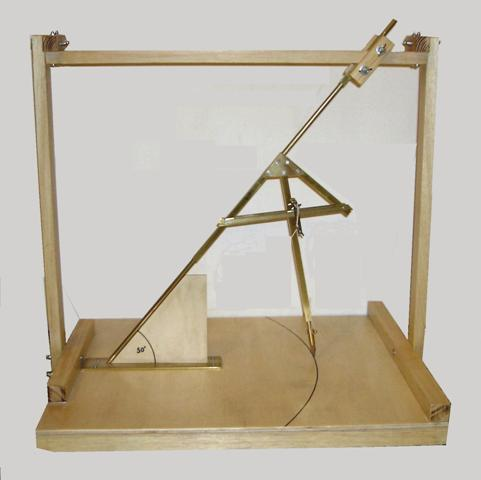
\includegraphics[width=.9\textwidth,keepaspectratio=true]{perfect1.jpg}
\medskip
\caption{A perfect compass}\label{f.perfect-image1}
\end{center}
\end{minipage}
\hfill
\begin{minipage}{.55\textwidth}
\begin{center}
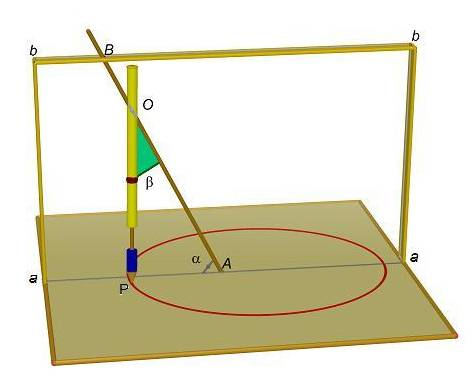
\includegraphics[width=\textwidth,keepaspectratio=true]{perfect2.jpg}
\caption{The configuration of a perfect compass}\label{f.perfect-image2}
\end{center}
\end{minipage}
\end{figure}

%\begin{figure}[h]
%\begin{center}
%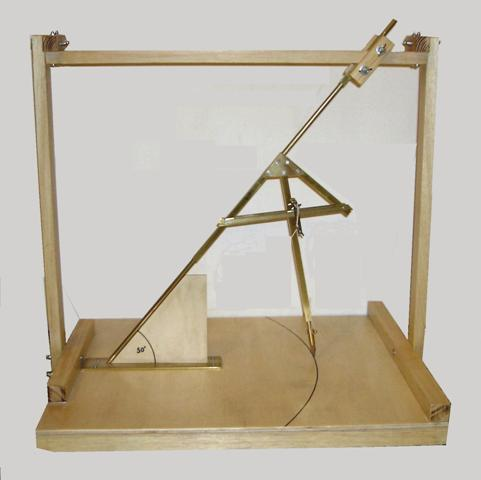
\includegraphics[width=.5\textwidth,keepaspectratio=true]{perfect1.jpg}
%\caption{A perfect compass}\label{f.perfect-image1}
%\end{center}
%\end{figure}
%\begin{figure}[h]
%\begin{center}
%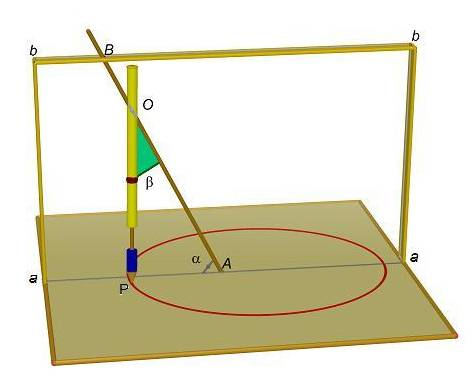
\includegraphics[width=.6\textwidth,keepaspectratio=true]{perfect2.jpg}
%\caption{The configuration of a perfect compass}\label{f.perfect-image2}
%\end{center}
%\end{figure}



The axis $AB$ is fixed to the base at $A$ at an angle $\alpha$. The arm is attached to the axis at $O$ at an angle $\beta$ and the pencil touches the bases at $P$. The parameters $\alpha, \beta, AB$ determine which conic section will be drawn. Here we limit ourselves to ellipses by specifying that $0< \beta <\alpha< 90$. 

The notation in the figures in the sequel conform to the notation in \cite{henk}. $B$ denotes the point of attachment of the to the axis while $O$ is reserved for the center of the conic section. The axis is drawn in red and the arm in blue.

%%%%%%%%%%%%%%%%%%%%%%%%%%%%%%%%%%%%%%%%%%%%%%%%%%%%%%%%%%%%%

\subsubsection*{Constructing the major axis}


Consider an arbitrary point $A$ on an arbitrary line $l$ that we have drawn to be horizontal (Figure~\ref{f.perfect-major}). Place the base of the axis $AB$ at $A$ and rotate the axis until the arm intersects the line $l$. There are two intersections labeled $E$ and $D$. Let the midpoint of $ED$ be $O$. Construct the (outer) circle centered at $O$ with radius $OD=OE=r_o$.

The diagrams will be drawn in two dimensions; you have to imagine that $B$ is actually above the plane and the axis $AB$ and the arms $BD, BE$ have been ``laid flat.''

%%%%%%%%%%%%%%%%%%%%%%%%%%%%%%%%%%%%%%%%%%%%%%%%%%%%%%%%%%%%%

\begin{figure}
\begin{minipage}{.49\textwidth}
\begin{center}
\begin{tikzpicture}[scale=.8]
\clip  (-3.9,-3.6) rectangle +(9,7.2);

\def\alph{50}
\def\bet{30}
\def\len{3.5}

\path[name path=major] (-6,0) -- (10,0);
\coordinate (A) at (2,0);
\node[below right] at (A) {$A$};
\draw[thick,red] (A) --  +({\alph}:{\len}) coordinate (B);
\path[thick,name path=arm1] (B) -- +({180+\alph-\bet}:12);
\node[above] at (B) {$B$};

\path [name intersections = {of = arm1 and major, by = {E}}];
\node[below left] at (E) {$E$};

\draw[blue,thick] (B) -- (E);

\path[thick,name path=arm2] (B) -- +({180+\alph+\bet}:6);
\path [name intersections = {of = arm2 and major, by = {D}}];
\node[below right] at (D) {$D$};

\draw[blue,thick] (B) -- (D);

\coordinate (O) at ($(E)!.5!(D)$);
\node[below left] at (O) {$O$};
\node[draw,thick,dashed,name path=circle] at (O) 
  [circle through = (D)] {};
\draw ($(E)+(-36pt,0)$) -- ($(D)+(36pt,0)$) node[xshift=-2pt,above] {$l$};
\path (E) -- node[below] {$r_o$} (O);

\node[above right,xshift=3pt] at (A) {\sm{\alpha}};
\node[above left,xshift=5pt] at (A) {\sm{180\!-\!\alpha}};
\node[below left,xshift=-10pt,yshift=-5pt] at (B) {\sm{\beta}};
\node[below left,xshift=-1pt,yshift=-7pt] at (B) {\sm{\beta}};
\vertexsm{O};

\end{tikzpicture}
\caption{Constructing the major axis}\label{f.perfect-major}
\end{center}
\end{minipage}
%\end{figure}
\hfill
%\begin{figure}[t]
\begin{minipage}{.49\textwidth}
\begin{center}
\begin{tikzpicture}[scale=.8]
\clip  (-3.7,-3.6) rectangle +(9.4,7.2);

\def\alph{50}
\def\bet{30}
\def\len{3.5}

\path[name path=major] (-6,0) -- (10,0);
\coordinate (A) at (2,0);
\node[below right] at (A) {$A$};
%\draw[thick,red] (A) -- +({\alph}:{\len}) coordinate (B);
\path[thick,name path=arm1] (B) -- +({180+\alph-\bet}:12);
%\node[above] at (B) {$B$};

\path [name intersections = {of = arm1 and major, by = {E}}];
\node[below left] at (E) {$E$};

%\draw[blue,thick] (B) -- (E);
\draw (E) -- (A);

\path[thick,name path=arm2] (B) -- +({180+\alph+\bet}:6);
\path [name intersections = {of = arm2 and major, by = {D}}];
\node[below right] at (D) {$D$};

%\draw[blue,thick] (B) -- (D);

\coordinate (O) at ($(E)!.5!(D)$);
\node[below left] at (O) {$O$};
\node[draw,thick,dashed,name path=circle] at (O) 
  [circle through = (D)] {};

\draw[thick,red] (A) -- +({\len},0) coordinate (U);
\node[below] at (U) {$U$};

\path[name path=arm3] (U) -- +({180+\bet}:7);
\path[name path=perp] (A) -- +(-90:5);

\path [name intersections = {of = arm3 and perp, by = {G}}];
\node[below right] at (G) {$G$};
\draw[thick,blue] (U) -- (G);
\path [name intersections = {of = perp and circle, by = {K}}];
\node[below] at (K) {$K$};
\draw (A) -- (K);
\draw[name path=ko] (O) -- node[above right,xshift=-4pt] {$r_o$} (K);
\path[name path=gl] (G) -- +(180:4);
\path [name intersections = {of = ko and gl, by = {L}}];
\node[below,xshift=-3pt,yshift=-5pt] at (L) {$L$};
\draw (G) -- (L);

\node[draw,thick,dotted,name path=inner] at (O)   
  [circle through = (L)] {};

\path[name path=minor] ($(O)+(0,4)$) -- ($(O)+(0,-4)$);
\path [name intersections = {of = minor and inner, by = {H,T}}];
\node[above] at (H) {$H$};
\node[below] at (T) {$T$};

\draw (H) -- node[left] {$r_i$} (O) -- node[left] {$r_i$} (T);

\node[above,xshift=-3pt,yshift=5pt] at (K) {\sm{\beta}};
\node[below left,xshift=-12pt,yshift=1pt] at (U) {\sm{\beta}};
%\vertexsm{G};
\draw[rotate=180] (G) rectangle +(5pt,5pt);
\draw[rotate=180] (A) rectangle +(5pt,5pt);
\draw[rotate=90] (O) rectangle +(5pt,5pt);
\end{tikzpicture}
\caption{Constructing the minor axis}\label{f.perfect-minor}
\end{center}
\end{minipage}
\end{figure}

%%%%%%%%%%%%%%%%%%%%%%%%%%%%%%%%%%%%%%%%%%%%%%%%%%%%%%%%%%%%%

\subsubsection*{Constructing the minor axis}

Consider now the situation where axis is rotated by $-90^\circ$ and denote by $G$ the intersection of the arm with the plane. If you lay the compass flat, the axis $AB$ becomes $U$ (Figure~\ref{f.perfect-minor}). Extend $AG$ until it intersects the circle at $K$ and construct $OK=r_o$. Construct the perpendicular to $AK$ at $G$ and let its intersection with $OK$ be $L$. Draw the (inner) circle centered at $O$ with radius $OL=r_i$. Construct the perpendicular to $ED$ at $O$ and let its intersections with the inner circle be $H,T$.

\begin{theorem}[Prop. VIII]
$\displaystyle\frac{AG}{AK}=\frac{HO}{OD}$, where $HO=r_i$ and $OD=r_o$ are the semi-minor and semi-major axes of an ellipse.
\end{theorem}
\begin{proof}
By Theorem~\ref{thm.ratios-besant},
\[
\frac{AG^2}{DA\cdot AE} = \frac{HO^2}{OD^2}\,,
\]
and by Theorem~\ref{thm.alt-hypo}, $AK^2=DA\cdot AE$ .\fqed
\end{proof}

\subsubsection*{$G$ is a point the ellipse with semi-major axis $r_o$ and semi-minor axis $r_i$}

Since $\triangle AKO \sim \triangle AGO$,
\[
\frac{AG}{AK}=\frac{OL}{OK}=\frac{r_i}{r_o}=\frac{HO}{OD}\,,
\]
and $G$ is a point on an ellipse with semi-minor axis $r_i$ and semi-major axis $r_o$.

%%%%%%%%%%%%%%%%%%%%%%%%%%%%%%%%%%%%%%%%%%%%%%%%%%%%%%%%%%%%%

An alternate method of proving that $G$ is on an ellipse is to show that the coordinates of $G$ satisfy the parametric representation (Definition~\ref{def.parametric}). Let $t$ be the angle between $OD$ and $OK$. $OA=r_o\cos t$ and $AG=r_i\sin t$ (Figure~\ref{f.perfect-parametric}) so $G$ is a point on the ellipse. 

Figure~\ref{f.perfect-ellipse} shows the ellipse (green) and you can check that $G$ is on the ellipse. It also shows that a symmetric construction gives the point $G'$ on the ellipse. Another symmetric construction shows that there are an additional pair of points to the left of the minor-axis.  An easy way to see this is that moving $A$, the base of the axis to the symmetrical position on $OE$ will cause the same curve to be constructed. We have now located six points on an ellipse. Form the following surprising theorem (proof omitted) we conclude that the perfect compass constructs an ellipse.\footnote{Approaches to proving the theorem are discussed in the Wikipedia article \emph{Five points determine a conic}.}

%%%%%%%%%%%%%%%%%%%%%%%%%%%%%%%%%%%%%%%%%%%%%%%%%%%%%%%%%%%%%

\begin{figure}
\begin{minipage}{.49\textwidth}
\begin{center}
\begin{tikzpicture}[scale=.8]
\clip (-3.8,-3.6) rectangle +(8.4,7.2);

\def\alph{50}
\def\bet{30}
\def\len{3.5}

\path[name path=major] (-6,0) -- (10,0);
\coordinate (A) at (2,0);
\node[below right] at (A) {$A$};
%\draw[thick,red] (A) -- +({\alph}:{\len}) coordinate (B);
\path[thick,name path=arm1] (B) -- +({180+\alph-\bet}:12);
%\node[above] at (B) {$B$};

\path [name intersections = {of = arm1 and major, by = {E}}];
\node[below left] at (E) {$E$};

%\draw[blue,thick] (B) -- (E);
\draw (E) -- (D);

\path[thick,name path=arm2] (B) -- +({180+\alph+\bet}:6);
\path [name intersections = {of = arm2 and major, by = {D}}];
\node[below right] at (D) {$D$};

\coordinate (O) at ($(E)!.5!(D)$);
\node[below left] at (O) {$O$};
\node[draw,thick,dashed,name path=circle] at (O) 
  [circle through = (D)] {};

\path[name path=arm3] (U) -- +({180+\bet}:7);
\path[name path=perp] (A) -- +(-90:5);

\path [name intersections = {of = arm3 and perp, by = {G}}];
\node[below right] at (G) {$G$};
%\draw[thick,blue] (U) -- (G);
\path [name intersections = {of = perp and circle, by = {K}}];
\node[below] at (K) {$K$};
\draw (A) -- (K);
\path[name path=ko] (O) -- (K);
%\draw[name path=ko] (O) -- node[above right,xshift=-4pt] {$r_o$} (K);
\path[name path=gl] (G) -- +(180:4);
\path [name intersections = {of = ko and gl, by = {L}}];
\node[below,xshift=-3pt,yshift=-5pt] at (L) {$L$};
\draw (G) -- (L);

\node[draw,thick,dotted,name path=inner] at (O)   
  [circle through = (L)] {};

\path[name path=minor] ($(O)+(0,4)$) -- ($(O)+(0,-4)$);
\path [name intersections = {of = minor and inner, by = {H,T}}];
\node[above] at (H) {$H$};
\node[below] at (T) {$T$};
\draw (H) -- node[left] {$r_i$} (O) -- node[left] {$r_i$} (T);

\draw[very thick,cyan] (O) -- node[xshift=-3pt,below,black] {$r_i$} (L);
\draw[very thick,brown] ($(O)+(4pt,0pt)$) --
   node[above,black,xshift=4pt] {$r_o$} ($(K)+(4pt,0pt)$);

\node[below right,xshift=10pt] at (O) {$t$};

\path (O) -- node[above] {$r_o\cos t$} (A);
\path (A) -- node[right,xshift=2pt] {$r_i\sin t$} (G);

\vertexsm{G};
\draw[rotate=180] (G) rectangle +(5pt,5pt);
\draw[rotate=180] (A) rectangle +(5pt,5pt);
\draw[rotate=90] (O) rectangle +(5pt,5pt);

\end{tikzpicture}
\caption{The parametric representation}\label{f.perfect-parametric}
\end{center}
\end{minipage}
%\end{figure}
%
%%%%%%%%%%%%%%%%%%%%%%%%%%%%%%%%%%%%%%%%%%%%%%%%%%%%%%%%%%%%%%
%
%\begin{figure}[b]
\hfill
\begin{minipage}{.49\textwidth}
\begin{center}
\begin{tikzpicture}[scale=.8]
\clip (-3.8,-3.6) rectangle +(8.3,7.2);

\def\alph{50}
\def\bet{30}
\def\len{3.5}

\path[name path=major] (-6,0) -- (10,0);
\coordinate (A) at (2,0);
\node[below right] at (A) {$A$};
\path[thick,red] (A) -- +({\alph}:{\len}) coordinate (B);
\path[thick,name path=arm1] (B) -- +({180+\alph-\bet}:12);
%\node[above] at (B) {$B$};

\path [name intersections = {of = arm1 and major, by = {E}}];
\node[below left] at (E) {$E$};

%\draw[blue,thick] (B) -- (E);

\path[thick,name path=arm2] (B) -- +({180+\alph+\bet}:6);
\path [name intersections = {of = arm2 and major, by = {D}}];
\node[below right] at (D) {$D$};

\path[blue,thick] (B) -- (D);
\draw (E) -- (D);

\coordinate (O) at ($(E)!.5!(D)$);
\node[below left] at (O) {$O$};
\node[draw,thick,dashed,name path=circle] at (O) 
  [circle through = (D)] {};

\path[thick,red] (A) -- +({\len},0) coordinate (U);
%\node[below] at (U) {$U$};

\path[name path=arm3] (U) -- +({180+\bet}:7);
\path[name path=perp] (A) -- +(-90:5);

\path[name path=arm3p] (U) -- +({180-\bet}:7);
\path[name path=perpp] (A) -- +(90:5);

\path [name intersections = {of = arm3 and perp, by = {G}}];
\node[below right] at (G) {$G$};
%\draw[thick,blue] (U) -- (G);

\path [name intersections = {of = arm3p and perpp, by = {GP}}];
\node[above right] at (GP) {$G'$};
%\draw[thick,blue] (U) -- (GP);

\path [name intersections = {of = perp and circle, by = {K}}];
\node[below] at (K) {$K$};
\draw (A) -- (K);

\path [name intersections = {of = perpp and circle, by = {KP}}];
\node[above] at (KP) {$K'$};
\draw (A) -- (KP);

\draw[name path=ko] (K) -- (O);
\path[name path=gl] (G) -- +(180:4);
\path [name intersections = {of = ko and gl, by = {L}}];
\node[below,xshift=-3pt,yshift=-5pt] at (L) {$L$};
\draw (G) -- (L);

\draw[name path=kop] (KP) -- (O);
\path[name path=glp] (GP) -- +(180:4);
\path [name intersections = {of = kop and glp, by = {LP}}];
\node[above,xshift=-3pt,yshift=5pt] at (LP) {$L'$};
\draw (GP) -- (LP);

\node[draw,thick,dotted,name path=inner] at (O)   
  [circle through = (L)] {};

\path[name path=minor] ($(O)+(0,4)$) -- ($(O)+(0,-4)$);
\path [name intersections = {of = minor and inner, by = {H,T}}];
\node[above] at (H) {$H$};
\node[below] at (T) {$T$};
\draw (H) -- (T);

\draw[name path=ellipse,very thick,green!80!black] (O)
  let
    \p1 = ($(O) - (D)$),
    \n1 = {veclen(\x1, \y1)},
    \p2 = ($(O) - (H)$),
    \n2 = {veclen(\x2, \y2)}
  in ellipse[x radius=\n1,y radius= \n2];

\vertexcolor{G}{green!80!black};
\vertexcolor{GP}{green!80!black};
\vertexcolor{E}{green!80!black};
\vertexcolor{D}{green!80!black};

\end{tikzpicture}
\caption{Checking that $G$ is on the ellipse}\label{f.perfect-ellipse}
\end{center}
\end{minipage}
\end{figure}

Add to sources and bibliography:

Section~\ref{s.perfect} is based on \cite{henk}; the authors develop formulas for computing the parameters of the ellipse drawn by a compass with given $AB,\alpha,\beta$, and conversely.

\begin{verbatim}
@unpublished{henk,
  author={Henk Hietbrink and Hazal Yürük},
  title={Why do we need a conic-section compass?},
  howpublished={submitted},
  year={2024},
}
\end{verbatim}


\end{document}
